\documentclass[conference]{IEEEtran}

\usepackage[utf8]{inputenc}
\usepackage[T1]{fontenc}
\usepackage[brazil]{babel}
\usepackage{amsmath,amssymb,amsfonts}
\usepackage{graphicx}
\usepackage{booktabs}
\usepackage{xcolor}

\begin{document}

\title{Modelos de Regressão e Classificação Linear Aplicados a Dados de PIB e Eletromiografia}

\author{
\IEEEauthorblockN{NOME DO(A) ALUNO(A) / NOMES DA EQUIPE}
\IEEEauthorblockA{
Universidade de Fortaleza -- UNIFOR\\
Inteligência Artificial Computacional\\
Fortaleza, Brasil\\
MATRÍCULA(S) -- E-MAIL(S)}
}

\maketitle

\begin{abstract}
Este trabalho apresenta a implementação de modelos de regressão e classificação
baseados no método dos mínimos quadrados. Na primeira etapa, foram usados dados do
Produto Interno Bruto da China para comparar o MQO tradicional, sua versão
regularizada e uma regressão polinomial. Na segunda etapa, sinais de
eletromiografia de dois músculos faciais foram empregados na classificação de
cinco expressões. Todos os modelos foram implementados com operações matriciais em
NumPy, seguindo os exemplos desenvolvidos em sala. A avaliação foi realizada por
amostragem aleatória, com 500 divisões de 80\% para treino e 20\% para teste. O
modelo polinomial apresentou os melhores resultados nas duas tarefas, alcançando
$R^2$ médio de 0,9949 na regressão e acurácia média de 99,28\% na classificação.
\end{abstract}

\begin{IEEEkeywords}
mínimos quadrados, regressão polinomial, regularização de Tikhonov,
classificação, eletromiografia
\end{IEEEkeywords}

\section{Introdução}

Modelos lineares são uma forma simples de estudar a relação entre variáveis. Em
um problema de regressão, a saída é numérica e contínua; em classificação, a
saída representa uma categoria. Apesar dessa diferença, os dois casos podem ser
tratados por uma formulação semelhante quando a classificação é organizada como
um problema de múltiplas saídas \cite{bishop,james}.

O trabalho foi dividido em duas partes. A primeira utiliza o ano para estimar o
PIB da China. A segunda utiliza medidas de dois sensores musculares para
identificar cinco expressões faciais. Em ambos os casos foram comparados o método
dos mínimos quadrados ordinários (MQO), o MQO regularizado e uma extensão
polinomial. O objetivo foi observar não apenas o valor médio das métricas, mas
também sua variação quando os conjuntos de treino e teste são alterados.

\section{Metodologia}

\subsection{Organização e preparação dos dados}

O conjunto de regressão contém 55 observações entre 1960 e 2014. A matriz $X$
possui uma coluna, correspondente ao ano, e o vetor $y$ contém o PIB em dólares.
O conjunto de eletromiografia contém 50.000 observações, distribuídas igualmente
entre cinco classes. As duas primeiras colunas correspondem aos sensores e a
terceira informa a expressão facial.

As entradas foram padronizadas por z-score. Para uma característica $x$, foi
aplicada a transformação

\begin{equation}
z = \frac{x-\mu_{\mathrm{treino}}}{\sigma_{\mathrm{treino}}}.
\label{eq:zscore}
\end{equation}

A média e o desvio-padrão foram calculados somente no conjunto de treino. Essa
separação evita que informações do conjunto de teste participem do ajuste e
também reduz problemas numéricos causados pelas potências das entradas.

\subsection{MQO e regularização}

Com o intercepto incluído, o modelo estima a saída por
$\hat{Y}=\Phi\boldsymbol{\beta}$, onde $\Phi$ é a matriz de projeto. Os parâmetros
do MQO foram obtidos pelas equações normais:

\begin{equation}
\boldsymbol{\beta} =
(\Phi^{T}\Phi)^{\dagger}\Phi^{T}Y,
\label{eq:mqo}
\end{equation}

em que o símbolo $\dagger$ indica a pseudoinversa. A versão regularizada de
Tikhonov acrescenta uma penalidade controlada por $\lambda$:

\begin{equation}
\boldsymbol{\beta} =
(\Phi^{T}\Phi+\lambda I)^{\dagger}\Phi^{T}Y.
\label{eq:ridge}
\end{equation}

Foram avaliados os valores $\lambda\in\{0; 0,25; 0,5; 0,75; 1\}$ na tarefa de
regressão. Como $\lambda=0$ resulta no próprio MQO tradicional, essa configuração
foi demonstrada na análise dos parâmetros, mas não repetida na tabela final.

\subsection{Expansão polinomial}

Para permitir relações não lineares, a matriz de projeto foi expandida como

\begin{equation}
\Phi=[\mathbf{1},X,X^2,\ldots,X^q].
\label{eq:poly}
\end{equation}

Seguindo a implementação usada em sala, as potências foram calculadas
separadamente para cada característica, sem termos cruzados. Na regressão, ordens
de 1 a 10 foram comparadas pelo $R^2$ médio em 50 divisões preliminares. Na
classificação, foram testadas ordens de 1 a 6, considerando a acurácia e o tempo
de ajuste. Quando duas ordens apresentaram desempenho muito próximo, foi mantida
a mais simples.

\subsection{Classificação multiclasse}

Os rótulos foram transformados em uma matriz $Y\in\mathbb{R}^{N\times C}$. A
coluna da classe correta recebeu $+1$ e as outras receberam $-1$. Depois do
ajuste, o modelo gerou cinco escores para cada amostra. A classe associada ao maior
escore foi escolhida com a operação $\operatorname{argmax}$.

\subsection{Procedimento de validação}

Foi utilizada validação por amostragem aleatória. Em cada uma das 500 rodadas, os
dados foram embaralhados e divididos em 80\% para treino e 20\% para teste. Na
regressão foram armazenados o erro quadrático médio (MSE) e o coeficiente de
determinação ($R^2$). Na classificação foi armazenada a acurácia. Ao final foram
calculados média, desvio-padrão, maior e menor valor de cada métrica.

\section{Resultados e Discussão}

\subsection{Regressão do PIB}

A Fig.~\ref{fig:regmodelos} mostra que os dados não seguem uma tendência retilínea.
O crescimento é relativamente lento nas primeiras décadas e acelera de forma
acentuada no final da série. Por esse motivo, as retas do MQO tradicional e do
regularizado ficam distantes de boa parte das observações. Mesmo um polinômio de
ordem 3, usado apenas nessa visualização inicial, já acompanha melhor a curvatura.

\begin{figure}[htbp]
\centerline{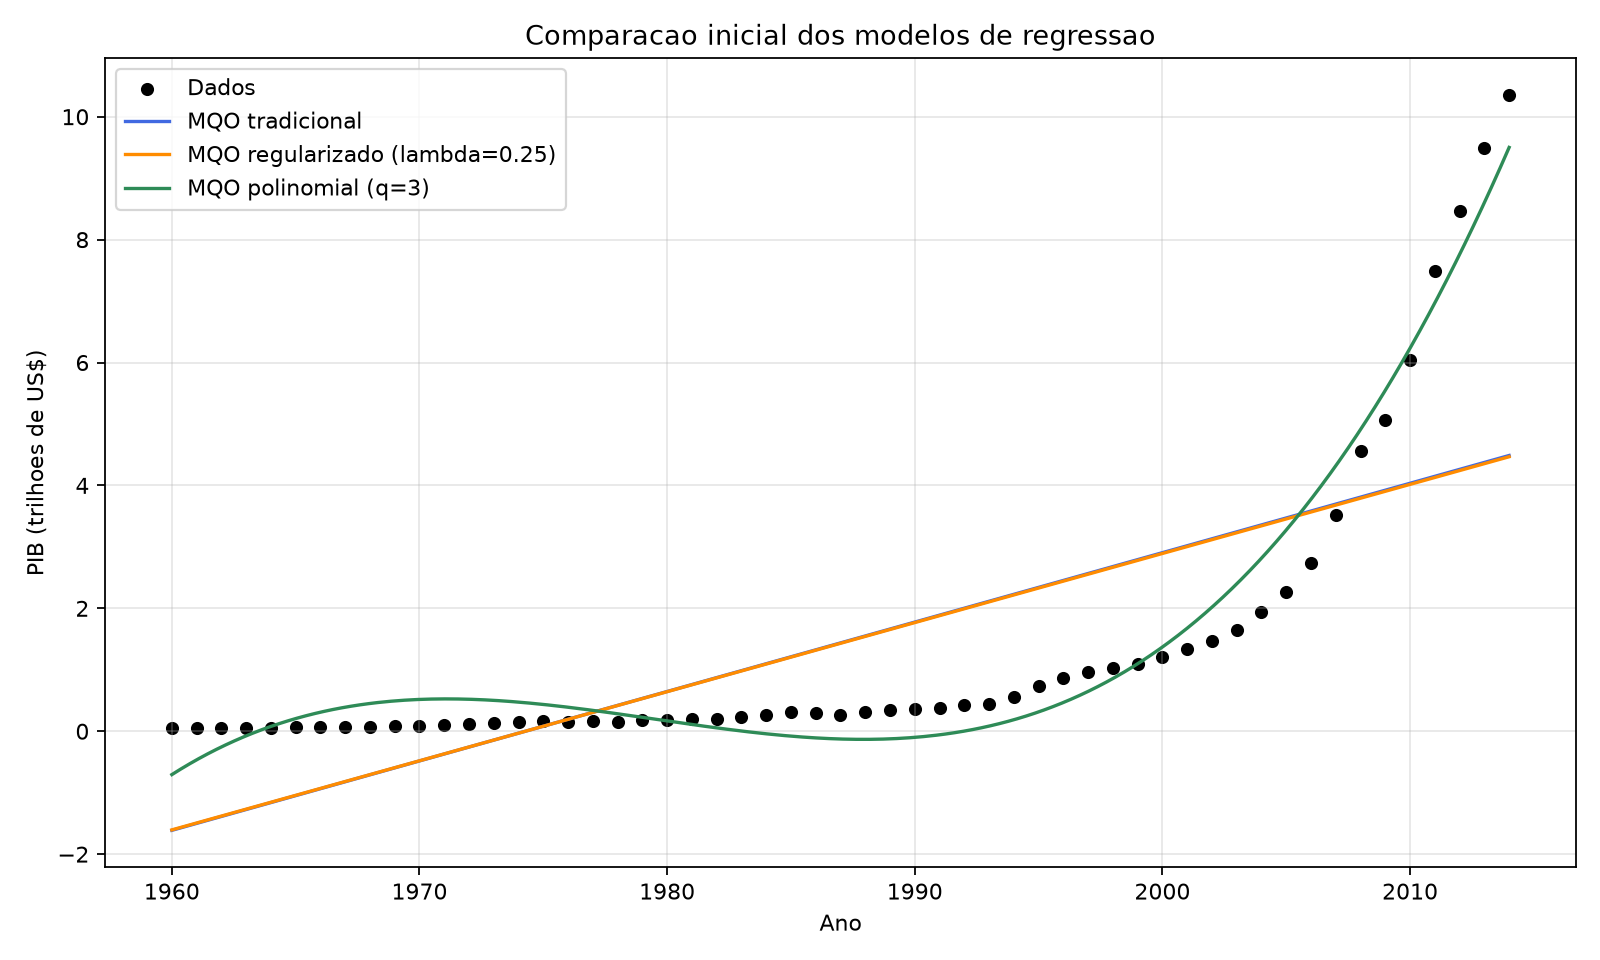
\includegraphics[width=\columnwidth]{../trabalho_av1/resultados/regressao/03_modelos_iniciais.png}}
\caption{Comparação inicial dos modelos para os dados de PIB.}
\label{fig:regmodelos}
\end{figure}

Na etapa de poda, o melhor resultado médio foi obtido com $q=9$, cujo $R^2$
preliminar foi 0,9965. A ordem 10 não melhorou o desempenho e apresentou uma
dispersão ligeiramente maior. Assim, o termo adicional não foi mantido.

A Tabela~\ref{tab:regressao} resume as 500 rodadas. O modelo polinomial alcançou
$R^2$ médio de 0,9949 e apresentou um MSE mais de duas ordens de grandeza menor
que os modelos lineares. Os valores negativos de $R^2$ dos modelos lineares não
são erro de cálculo: eles indicam que, em várias partições, a reta foi pior do que
uma previsão constante baseada na média do conjunto de teste.

\begin{table}[htbp]
\caption{Resultados médios da tarefa de regressão}
\label{tab:regressao}
\centering
\resizebox{\columnwidth}{!}{%
\begin{tabular}{lrrr}
\toprule
Modelo & MSE médio & $R^2$ médio & Desvio de $R^2$ \\
\midrule
Polinomial $q=9$ & $1,4544\times10^{22}$ & 0,9949 & 0,0145 \\
MQO tradicional & $3,3781\times10^{24}$ & -1,3214 & 9,5537 \\
Regularizado 0,25 & $3,3763\times10^{24}$ & -1,2942 & 9,4380 \\
Regularizado 0,50 & $3,3750\times10^{24}$ & -1,2676 & 9,3244 \\
Regularizado 0,75 & $3,3739\times10^{24}$ & -1,2415 & 9,2128 \\
Regularizado 1,00 & $3,3732\times10^{24}$ & -1,2160 & 9,1031 \\
\bottomrule
\end{tabular}}
\end{table}

A regularização diminuiu gradualmente a norma dos coeficientes e melhorou um
pouco o resultado da reta. Ainda assim, não corrigiu a principal limitação do
modelo: o formato linear é inadequado para a evolução observada do PIB.

\subsection{Classificação das expressões faciais}

Na Fig.~\ref{fig:emg}, cada cor representa uma expressão. As classes ocupam
regiões com formatos bastante diferentes. Algumas aparecem próximas aos eixos,
enquanto outras formam nuvens alongadas e parcialmente sobrepostas. Essa
disposição explica por que fronteiras exclusivamente retas encontram dificuldade
para separar todos os grupos.

\begin{figure}[htbp]
\centerline{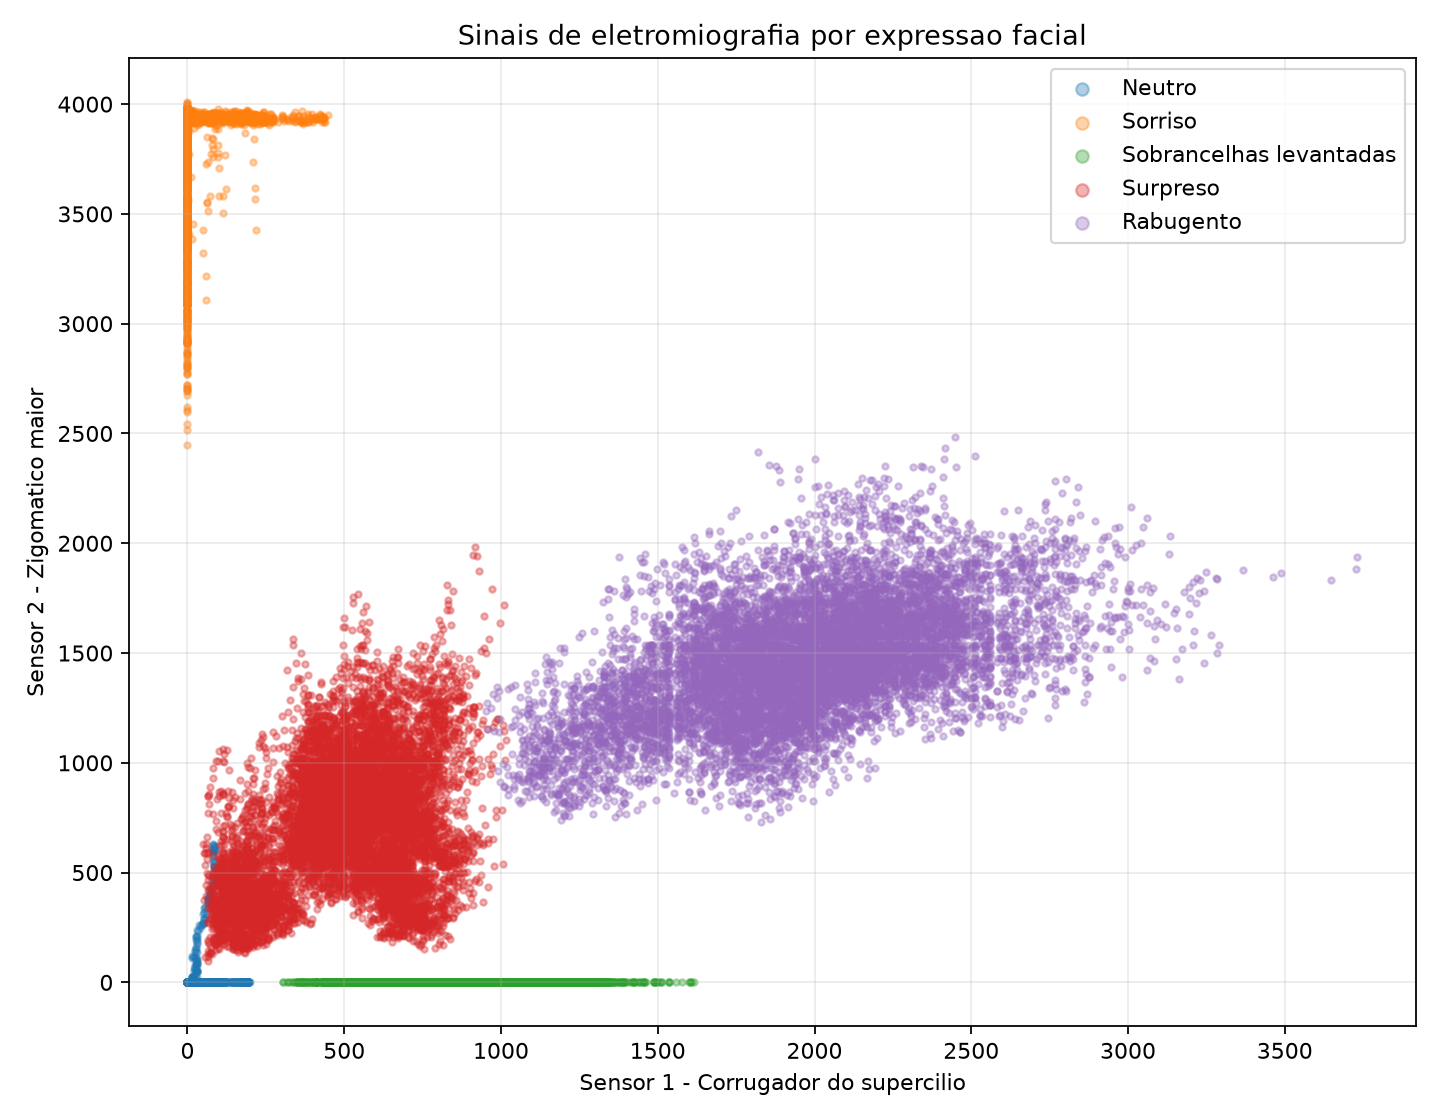
\includegraphics[width=\columnwidth]{../trabalho_av1/resultados/classificacao/02_dispersao_emg.png}}
\caption{Distribuição das cinco classes no espaço dos sensores.}
\label{fig:emg}
\end{figure}

As ordens 1, 2, 3, 4, 5 e 6 obtiveram acurácias preliminares de 72,53\%, 94,49\%,
97,64\%, 99,24\%, 99,26\% e 99,30\%, respectivamente. Foi selecionado $q=4$,
pois as duas ordens seguintes trouxeram ganhos menores que 0,1 ponto percentual,
ao mesmo tempo que aumentaram a quantidade de operações e o tempo de ajuste.

Os resultados finais aparecem na Tabela~\ref{tab:classificacao}. O modelo
polinomial manteve acurácia média de 99,28\% e desvio-padrão de apenas 0,083 ponto
percentual. Seu pior resultado entre as 500 rodadas ainda ficou acima de 99\%.

\begin{table}[htbp]
\caption{Resultados da tarefa de classificação}
\label{tab:classificacao}
\centering
\resizebox{\columnwidth}{!}{%
\begin{tabular}{lrrrr}
\toprule
Modelo & Média & Desvio & Maior & Menor \\
\midrule
MQO tradicional & 72,3888\% & 0,6430\% & 74,18\% & 70,13\% \\
Regularizado 0,25 & 72,3890\% & 0,6428\% & 74,18\% & 70,13\% \\
Polinomial $q=4$ & 99,2799\% & 0,0829\% & 99,48\% & 99,06\% \\
\bottomrule
\end{tabular}}
\end{table}

O MQO tradicional e o regularizado apresentaram resultados praticamente iguais.
Com 40.000 amostras de treino, a penalidade $\lambda=0,25$ é pequena em relação
aos valores acumulados em $\Phi^T\Phi$. Além disso, a regularização atua sobre os
coeficientes, mas não altera o fato de que as fronteiras continuam retas. A
expansão até a quarta ordem foi o que permitiu acompanhar a geometria das classes.

\begin{figure}[htbp]
\centerline{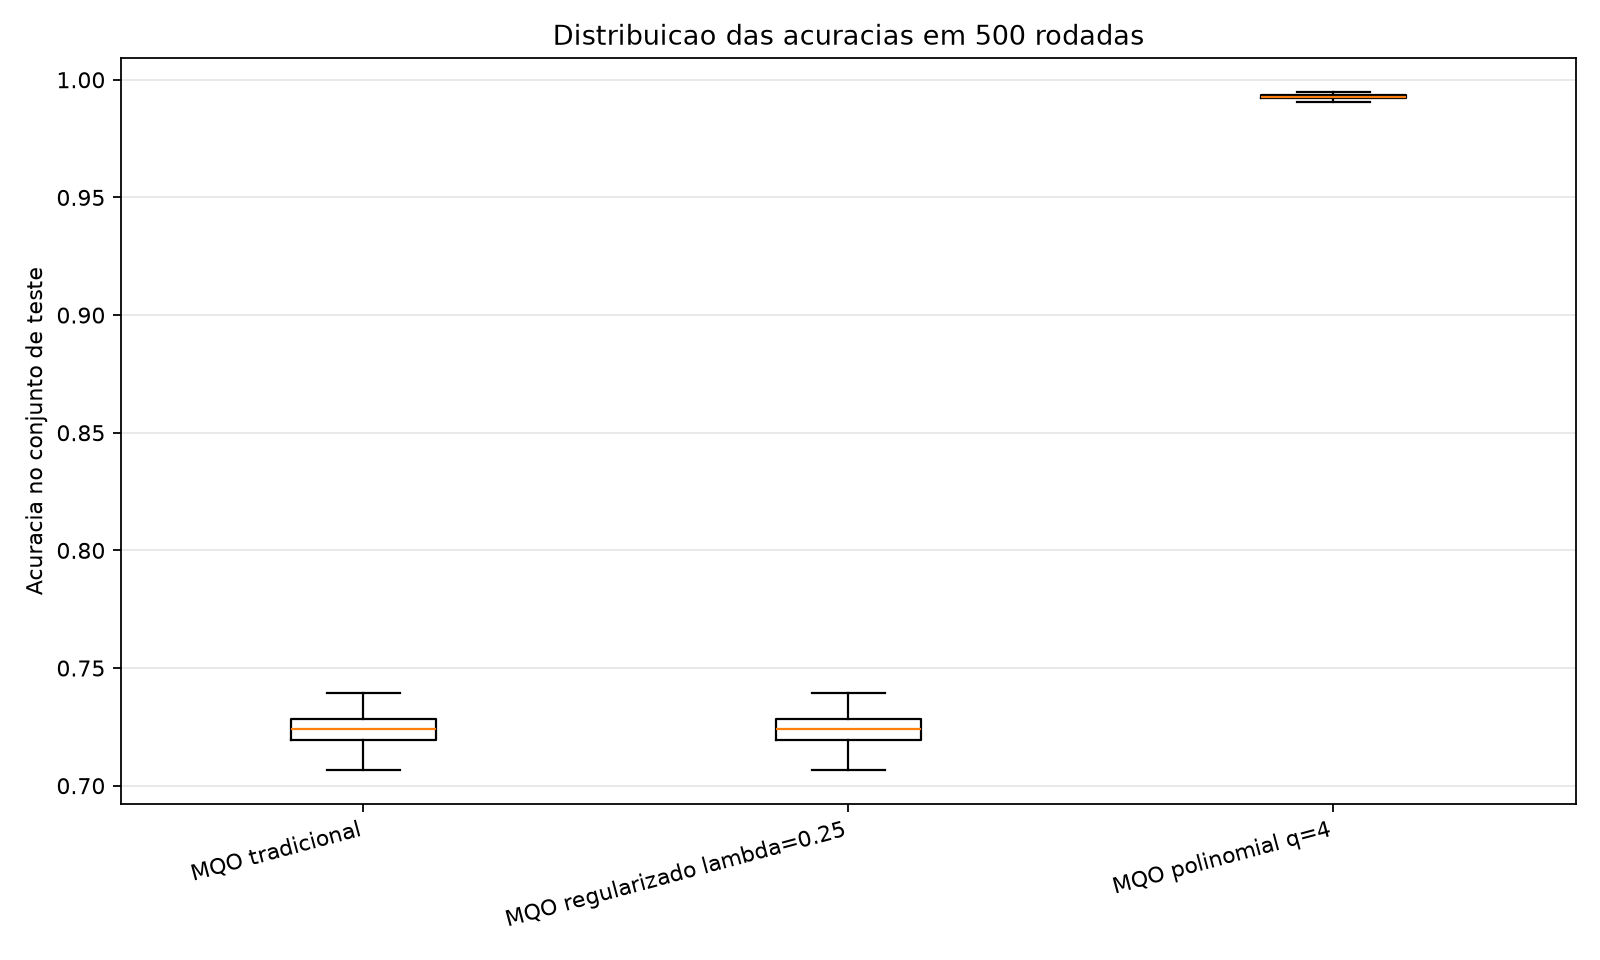
\includegraphics[width=\columnwidth]{../trabalho_av1/resultados/classificacao/06_distribuicao_acuracia.png}}
\caption{Distribuição das acurácias nas 500 rodadas.}
\label{fig:acuracias}
\end{figure}

\section{Conclusões}

Os experimentos mostraram que a escolha da forma do modelo teve maior impacto do
que a regularização nos dois conjuntos estudados. No problema do PIB, uma reta
não acompanhou o crescimento acelerado dos últimos anos, enquanto o polinômio de
ordem 9 obteve $R^2$ próximo de 1. Nos sinais musculares, as fronteiras lineares
alcançaram cerca de 72\% de acurácia, mas a expansão de ordem 4 elevou esse valor
para mais de 99\%.

A repetição das divisões de treino e teste foi importante para verificar se esses
resultados dependiam de uma única partição. O baixo desvio-padrão dos modelos
polinomiais indicou comportamento estável nas duas tarefas. Por fim, o trabalho
também mostrou que aumentar a complexidade indefinidamente não é necessário: as
ordens foram escolhidas somente enquanto os termos adicionais traziam melhoria
relevante.

\begin{thebibliography}{00}
\bibitem{bishop} C. M. Bishop, \textit{Pattern Recognition and Machine Learning}.
New York, NY, USA: Springer, 2006.
\bibitem{james} G. James, D. Witten, T. Hastie, and R. Tibshirani,
\textit{An Introduction to Statistical Learning}, 2nd ed. Springer, 2021.
\bibitem{aula} P. C. S. Barbosa, ``Fundamentos da regressão e classificação
linear,'' material didático da disciplina de Inteligência Artificial
Computacional, Universidade de Fortaleza.
\end{thebibliography}

\end{document}
